\section{Detector models}\label{sec:hist:detect}

One of the considerations we can gather from the previous Sections
is that
the problem of arrival time ---of a particle at a particular region of space---
can be tackled at different ``levels''.

Operationally, there must be a detector which
``clicks'' at the arrival of the particle, and the statistical distribution of
such click times over repeated measurements is studied. Due the Pauli objection,
probabilities in this distribution cannot simply be given in terms of projectors related to eigenspaces of a self-adjoint operator.
A more general formulation than projective measurement is therefore necessary.

Detectors can be treated (more or less explicitly) in quantum models of arrival time on different levels:
\begin{enumerate}
  \item
    Without making the detector explicit: this is the case of the Kijowski model \parencite{Kijowski, Leavens_TOA},
    which is based on positive-operator measures (POVM). Given there is no explicit detector in the model,
    the best candidate statistical distribution and operator are essentially obtained
    through consistency arguments, including a ``reasonable'' classical limit.
    See also the Aharonov--Bohm approach, described in Sec.~\ref{sec:AharonovBohm}.
  \item
    Phenomenological detector models:
    early attempts to incorporate the measurement apparatus
    (namely Allcock, Sec. \ref{sec:allcock}), which
    focus on the irreversible process of absorption.
    Normalization of the quantum state is not preserved, the Hamiltonian is not Hermitian
    because the potential is not real. The rate of normalization-loss is interpreted as
    absorption (or detection) probability over time.
    % The detector and the environment are fact
    % ``traced out'' and the particle is treated as an open system (Sec. \ref{sec:halliwell}).
  \item
    Full detector models: for example the Atom-Laser model. A two-level atoms in the ground state
    is sent to a laser-illuminated region (we are interested in the time-of-arrival into this region),
    is excited, and the first photon which is spontaneously emitted following the excitation
    is interpreted as detection of the arrival in the region. Problems related to
    reflection, low absorption rate, and delay in the spontaneous emission are fully taken into account in the model.
\end{enumerate}

A brief, mostly qualitative, illustration of the Atom-Laser model is
given below, and references therein can be consulted for more details.

\subsection{Basics of Atom-Laser Model}\label{sec:detect:atomlaser}

As pointed out in \cite{Damborenea}, the model by Halliwell (Sec. \ref{sec:halliwell})
has the merit of including irreversibility in the detection process,
but ``remains somewhat abstract
since no connection is made with any specific measuring
system''. The work by Damborenea et al. gives instead an operational
description of the notion of \emph{arrival time}.

The model describes an atom sent towards a laser-illuminated region.
The arrival time into the region is taken as the time\footnote{
  Please note, while there is an operational definition of detection,
  there is no operational definition of time; in other words,
  while this model does include an explicit description of the detector,
  there is still no description or definition of a ``clock''.
  % ,
  % which is still somewhat implicitly assumed as a ``classical'' one.
  % This further motivates theories modeling quantum clocks instead,
  % as will be seen from Chapter \ref{ch:pw} on.
}
when the first photon is spontaneously emitted by the atom,
following its excitation by the laser.
The spontaneous photon emission is therefore the ``click'' of the detector.

% This time-of-arrival formulation has been shown in excellent numerical agreement
% with Kijowski axiomatic distribution.

There are ``delays'':
\begin{enumerate*}[label=\arabic*)]
  \item in the transition of the atom to the excited state, and
  \item in the spontaneous emission.
\end{enumerate*}
This cannot be addressed by simply increasing the laser intensity
(therefore shortening the excitation and decay time)
because this would lead to %
% elastic
reflection,
and the most likely outcome would be no detection and no absorption at all.
This is similar to the issue encountered, at a theoretical level,
by Allcock when the imaginary absorbing potential was too large.

A suitable detector configuration, therefore, will be based on \emph{weak driving},
but will need to have the delays compensated,
which can be achieved
by computing the
deconvolution with the decay time distribution of an atom at rest.

The weak driving regime is characterized by longer lifetimes.
However, in \cite{Damborenea}, it is shown that,
as a limit for shorter lifetimes,
the deconvoluted distribution converges
to
the probability current flux.
This is interesting because, on the other hand, in general,
the probability current cannot be used to derive a time of arrival
distribution, due to the backflow effect
---for instance in a one dimensional system, a superposition of only positive momentum eigenfunctions may still lead to a
negative current, as it was initially noted by Allcock himself \parencite{Allcock-3}.

A possible experimental implementation can be based on a \emph{3-level} atom,
which decades into an intermediate, metastable,
``sink'' state after emission \parencite{Metastable, TQM2}.
% so
% that the atom can't immediately be excited again.\footnote{
%   This motivates studying 3-level systems with
%   relational models as well, as we'll see in \ref{sec:pw3l}.
% }

The model is based on treating the laser classically
while the atom and the spontaneously emitted photons are
described with the \term{quantum jump} or \term{quatum trajectories}
approach: similar to what we have seen in Sec. \ref{sec:halliwell}.
% , tracing out the photon leads to an effective
% imaginary term in the potential, and to an effective
% wavefunction which does not conserve its norm.

% A number of techniques and symmetry assumptions are also employed
% to simplify the model and ultimately reduce it
% to a time-independent one-dimensional problem
% ---namely,
% the rotating wave approximation
% and
% a laser-adapted interaction picture.

The effective \term{conditional Hamiltonian} reads:
\begin{equation}\label{eq:eff_atom_laser_detect_H}
  {H}_{c} = \frac{\hat{p}^2}{2m} +
  \frac{\hbar}{2} \left(
    \begin{matrix}
      0 & 0\\
      0 & -\iu\gamma
    \end{matrix}
  \right)
  +
  \frac{\hbar}{2} \left(
    \begin{matrix}%
      0         & \Omega(x)\\
      \Omega(x) & -2\Delta
    \end{matrix}
  \right)
  \text{,}
\end{equation}
where $\gamma$ is the decay rate or \term{Einstein coefficient},
$\Omega(x) = \Hvsd{x}\Omega$ is the Rabi frequency (ideally assuming that the half-space $x>0$ is uniformly illuminated by the laser),
and $\Delta$ is the effective detuning including Doppler and recoil effects
---but the on-resonance case ($\Delta=0$) can be considered,
by setting normal incidence and adjusting the laser frequency
(more details in \cite{Damborenea} and \cite[\s 4.2]{TQM2}).

The Hamiltonian in \eqref{eq:eff_atom_laser_detect_H} has an imaginary term $\iu\gamma$
which makes the Hamiltonian $H_c$ non-Hermitian. Wavefunctions
evolve, according to the Schr\"odinger equation, while \emph{loosing normalization};
the rate $-\dv{\norm{\psi}^2}{t}$ is then interpreted as the probability density
of the atom arrival being detected at time $t$. If the norm $\norm{\psi}^2$ vanishes for $t\rightarrow+\infty$,
that means that the detection will certainly occur at some time.
But that limit can be finite, indicating a certain probability of never being detected
(for example due to reflection).

The detection (i.e. spontaneous emission of the first photon) is generally delayed
with respect to the actual arrival at the laser-illuminated region, due to the finite time
required for excitation and de-excitation. That needs to be compensated via deconvolution
with the evolution of an atom at rest. Simply adjusting the optical parameters
to shorten the excitation and emission times
would not be a solution as it would either increase reflection rate dramatically
or simply increase the probability that atoms pass through the region undetected.

Nonetheless, one can focus on the state transition of the atom itself i.e.
the ``arrival'' at the excited state of the atom from the ground state,
rather than the arrival at a particular region in space. This is the
focus of Sec. \ref{sec:hist:detect:kiukas} below.

The general atom--laser
model gives, anyway, an operational justification for the interest
in more idealized (and tractable) models too.

\subsection{Arrival in an excited level}\label{sec:hist:detect:kiukas}

The detection-by-absorption model in \cite{RuschhauptAbsorption}
is also based on a complex potential that, plugged into the Schr\"odinger equation,
leads to a non-unitary evolution of the state vector
(with loss of normalization).

Specifically, the Hamiltonian $\hat{H}$ is replaced by a $\hat{H} - i\hat{D}$
(with $\hat{D}$ self-adjoint, bounded, positive):
\begin{equation}\label{eq:schrod_complex_pot}
  \qty(\hat{H}  - i\hat{D})\ket{\psi(t)} = i\hbar\dv{t}\ket{\psi(t)}  \text{.}
\end{equation}

A two-level example is considered to provide a concrete example.
Starting from the paper, we now carry on some explicit calculations.

By setting, out of convenience, $\hbar = \omega = 1$
(with $\omega$ the characteristic frequency of the system),
and directly considering the parameters
that minimize the time--energy uncertainty product \parencite{RuschhauptAbsorption},
we have a non-Hermitian ``Hamiltonian''
$\mathit{K} = \hat{H} - i\hat{D}$ with
\begin{equation}\label{eq:complexpot}
  \mathit{K} = \hat{H} - i\hat{D} \repr
    \hbar\omega\left\{
      \left[\begin{matrix}0 & 1\\1 & 0\end{matrix}\right] -
      i \left[\begin{matrix}0 & 0\\0 & \gamma \end{matrix}\right]
    \right\}
\end{equation}
and $\gamma = 2\sqrt{2}$.

We take an initial state of $\ket{0}$
(or $\mqty[1\\0]$ in matrix form).

We then compute, symbolically, the non-unitary evolution
$\ket{\psi(t)} = e^{-i\mathit{K}t}\ket{0}$
with the aid of \term{SymPy} \parencite{comp:sympy} within a \term{Jupyter} \parencite{comp:jupyter} notebook
(see Appendix \ref{detector-model-kiukas-ruschhaupt-schmidt-werner} for all the details of the calculation).

Simplifying the result in Eq.~\eqref{eq:sympy:non-unitary-evol}, we have:
\begin{equation}
  \ket{\psi(t)} \repr e^{-\frac{\sqrt{2}}{t}} \mqty[
    \cos(\frac{\sqrt{2}}{2}t) + \sin(\frac{\sqrt{2}}{2}t)& \\
                     -i\sqrt{2} \sin(\frac{\sqrt{2}}{2}t)&
  ] \,\text{.}
\end{equation}

\begin{figure} %% https://tex.stackexchange.com/a/165730
  \centering
  \begin{subfigure}{0.49\textwidth}
    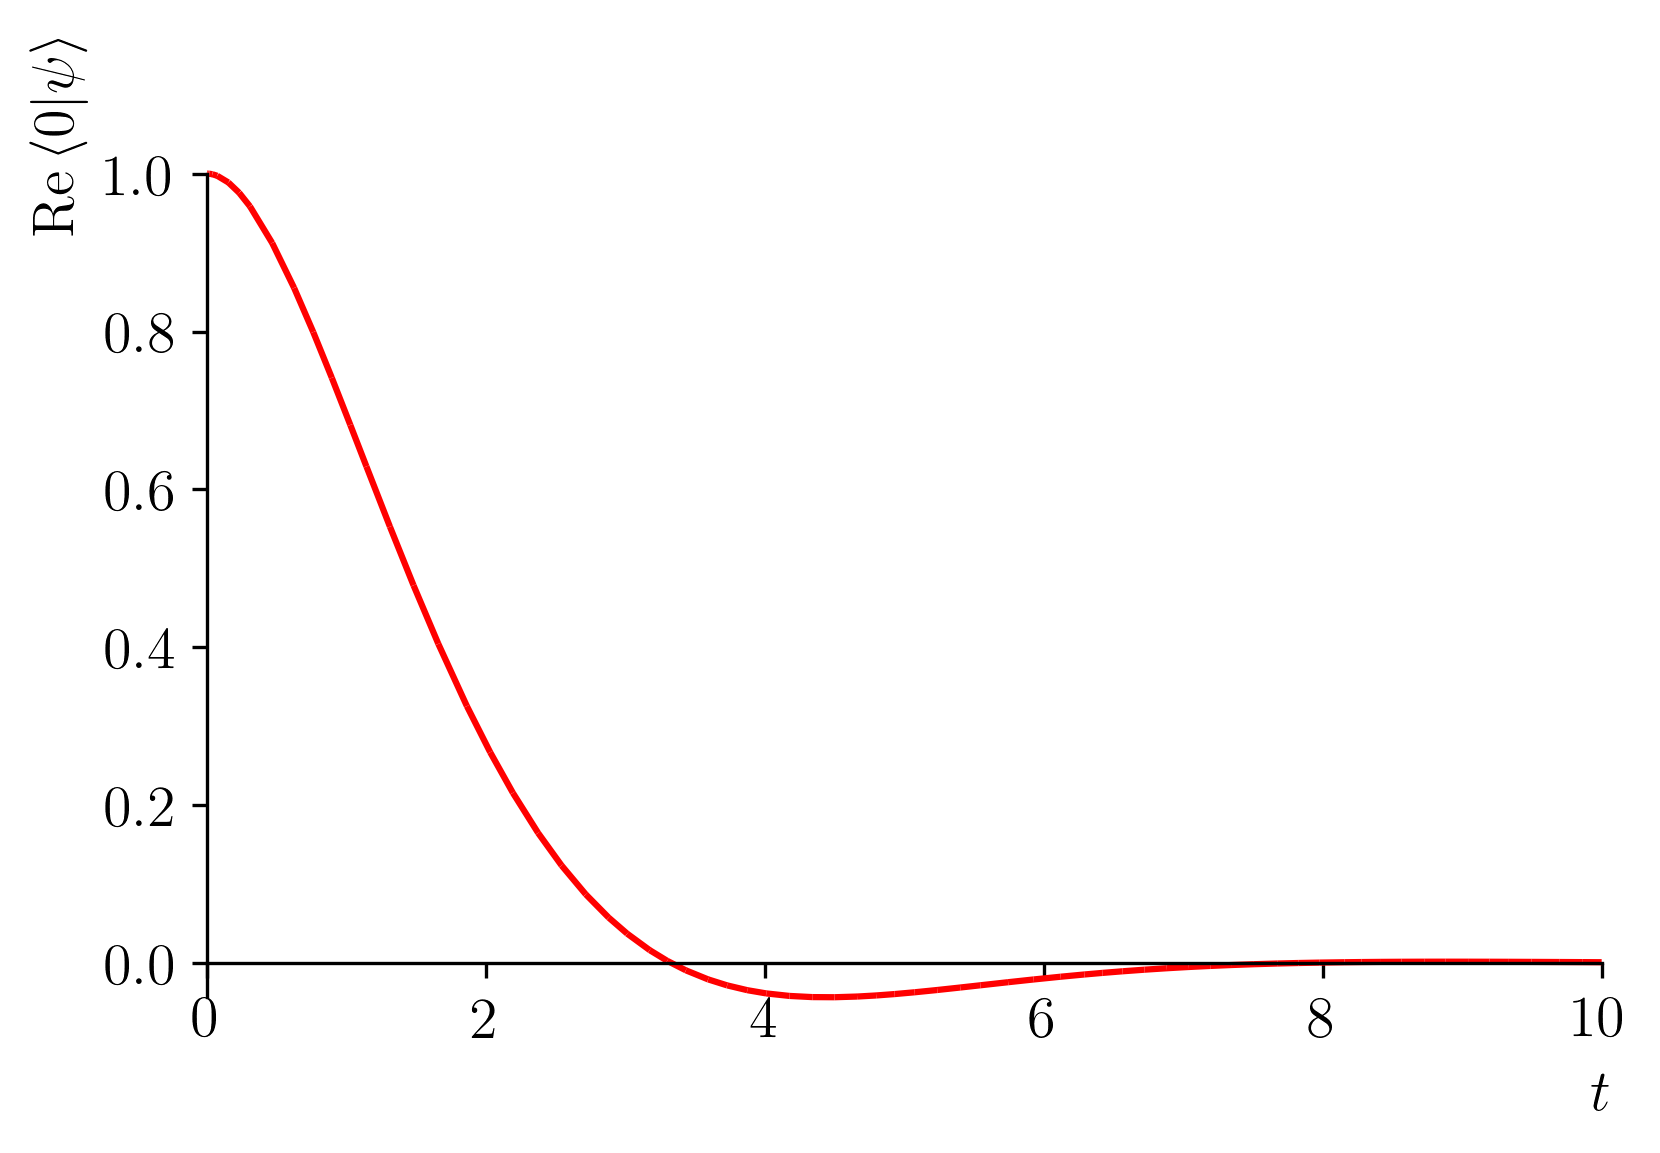
\includegraphics[width=\linewidth]{img/2ldetect/re_psi0_t.png}
    \subcaption{}\label{fig:absorbed-qubit-components:re0}
  \end{subfigure}
  % \hspace*{\fill} % separation between the subfigures
  \begin{subfigure}{0.49\textwidth}
    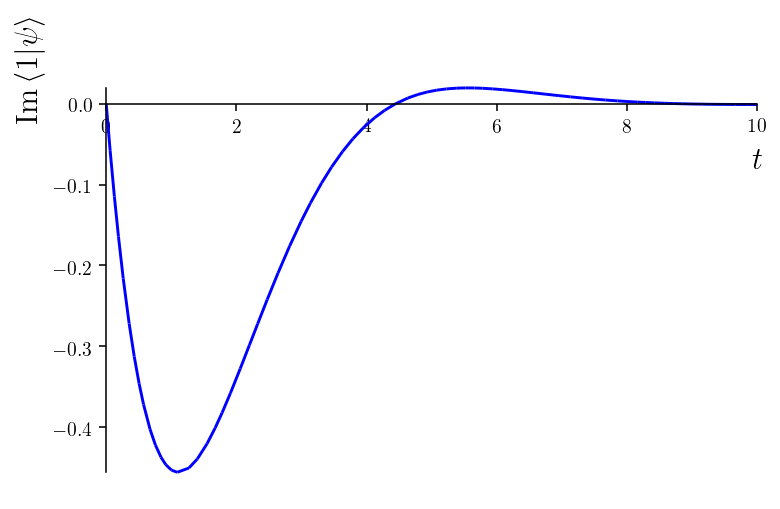
\includegraphics[width=\linewidth]{img/2ldetect/im_psi1_t.png}
    \subcaption{}\label{fig:absorbed-qubit-components:im1}
  \end{subfigure}
  % \hspace*{\fill} % separation between the subfigures
  \caption[
    Non-unitary evolution of absorbed qubit
  ]{
    Non-unitary evolution of the absorbed qubit
    according to the model in
    \cite{RuschhauptAbsorption}.
    The component along $\ket{0}$ is purely real,
    and the one along $\ket{1}$ is purely imaginary,
    therefore only their their respective parts are plotted.
  }\label{fig:absorbed-qubit-components}
\end{figure}

\begin{figure}
  \centering
  \begin{subfigure}[b]{0.49\textwidth}
    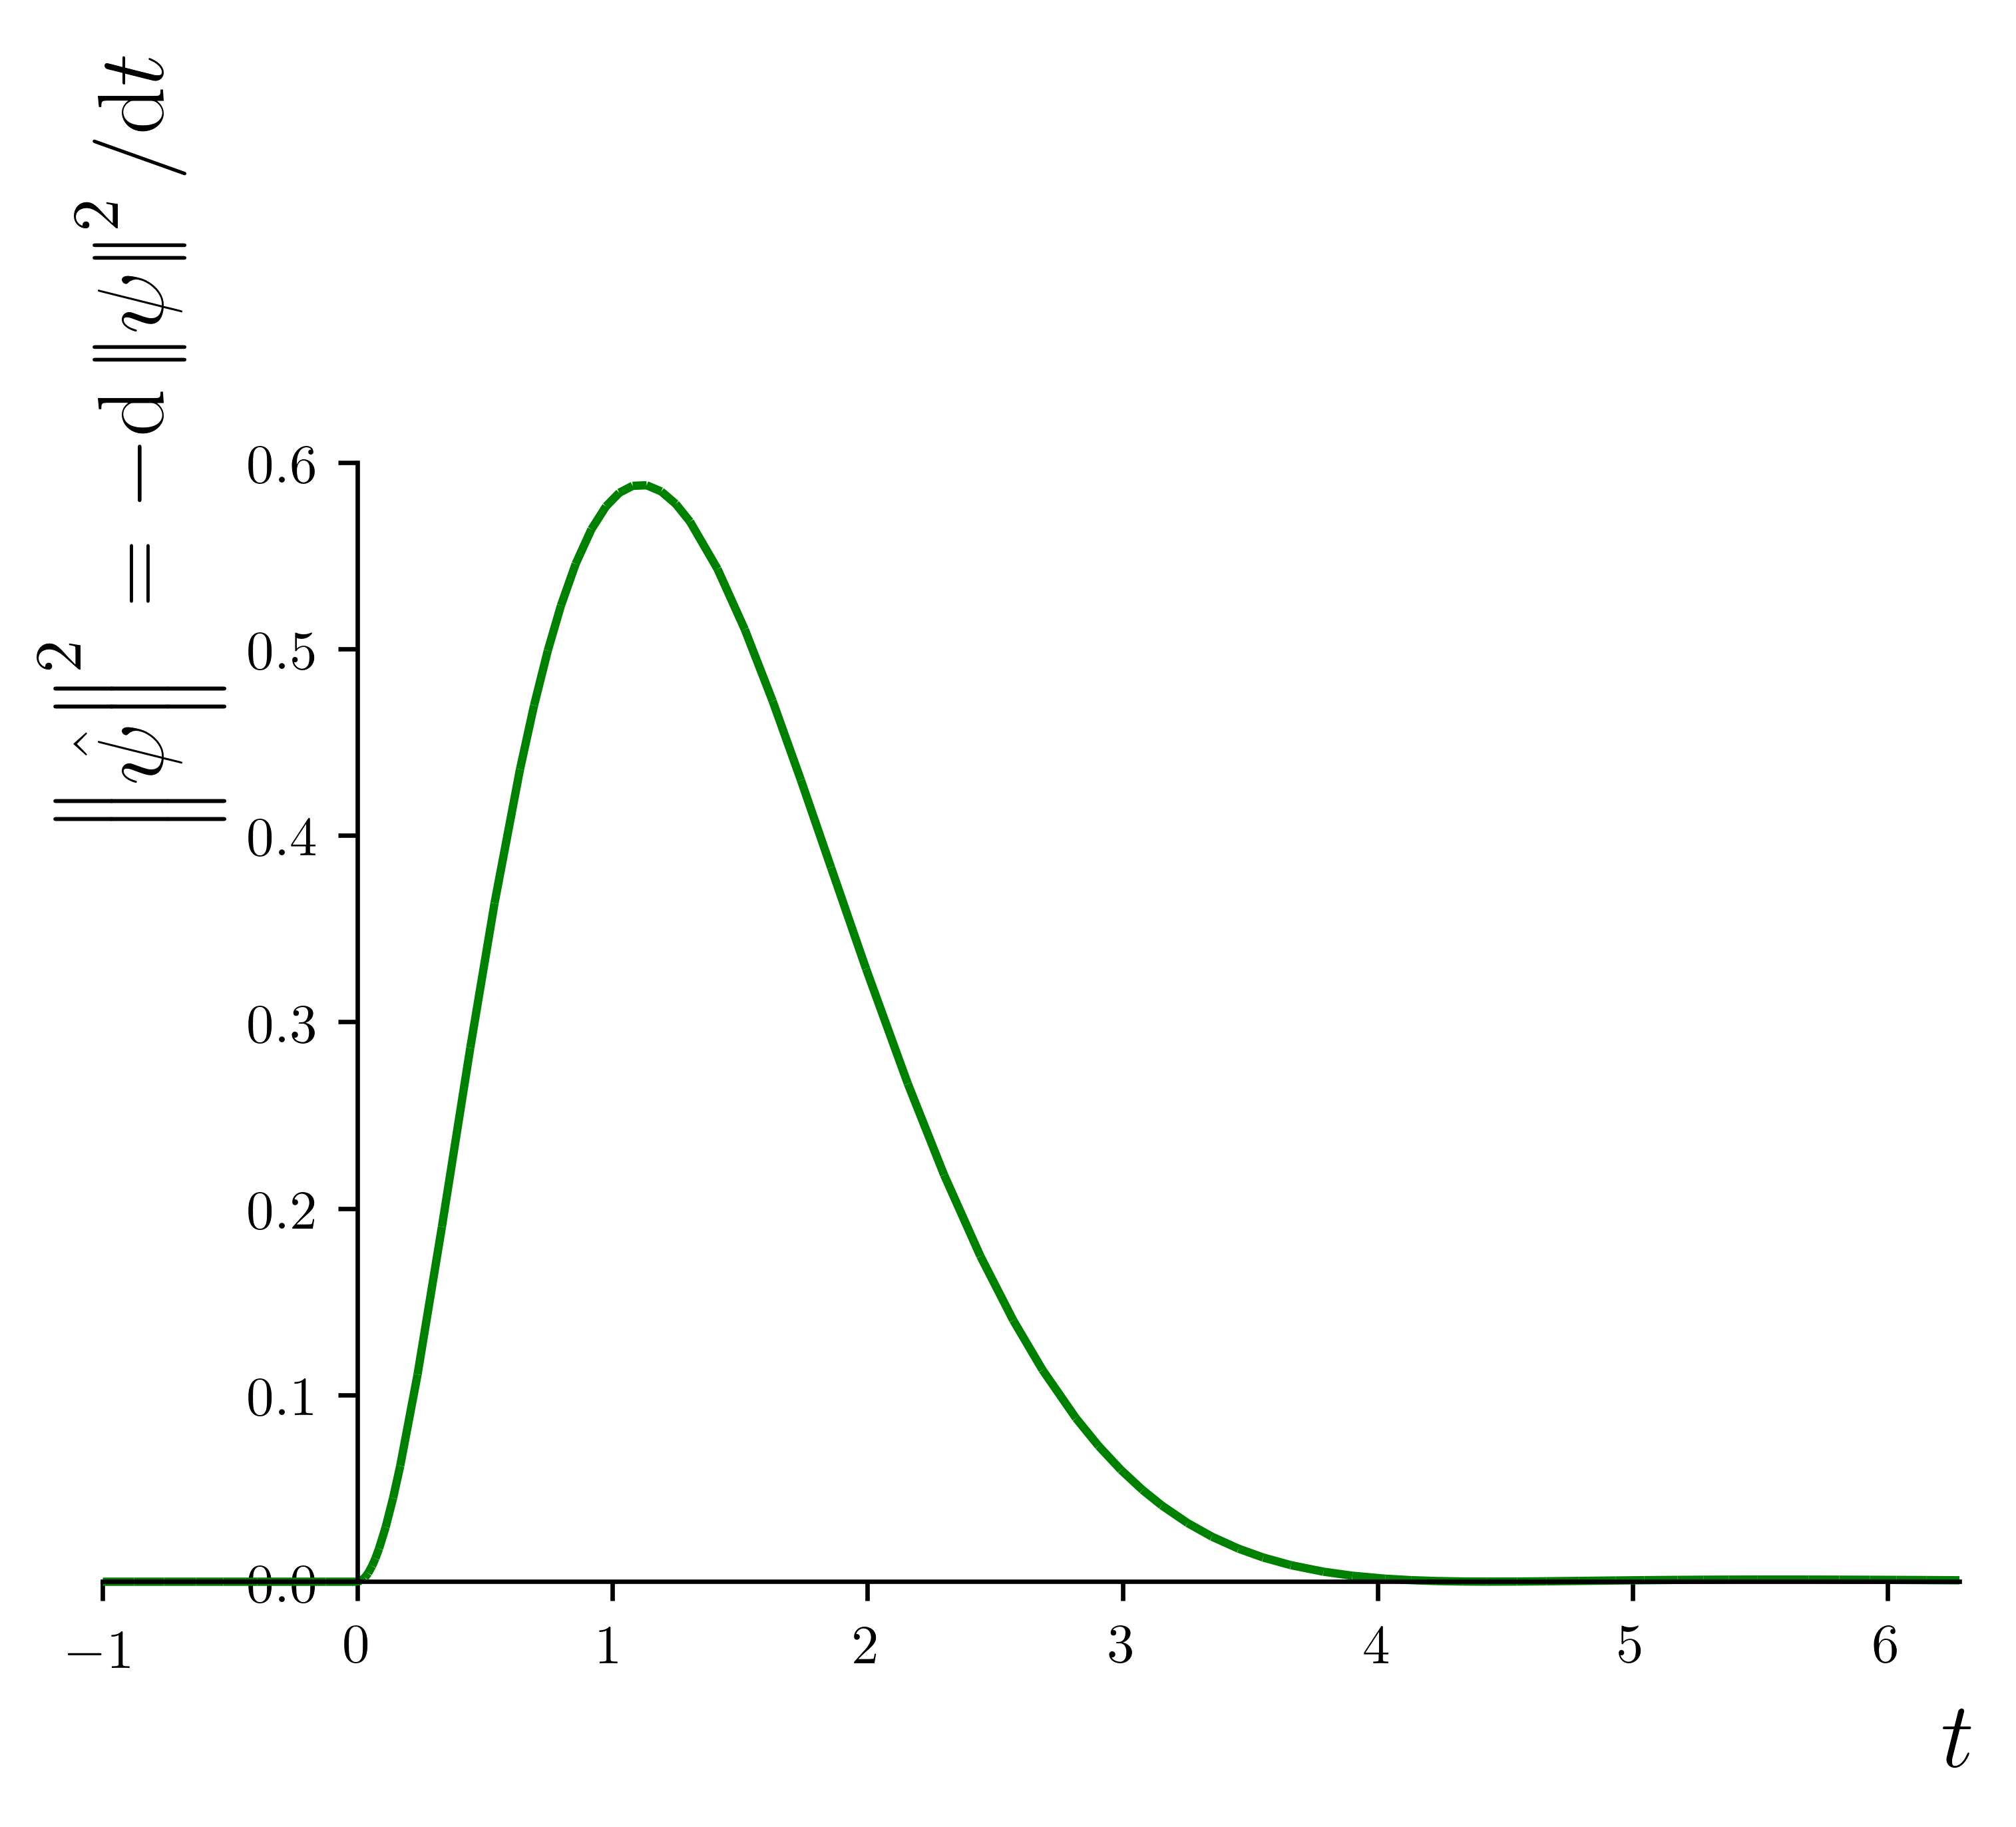
\includegraphics[width=\linewidth]{img/2ldetect/qubit_normalization_loss.png}
    \subcaption{}\label{fig:absorbed-qubit-normalization-loss:t}
  \end{subfigure}
  \begin{subfigure}[b]{0.49\textwidth}
    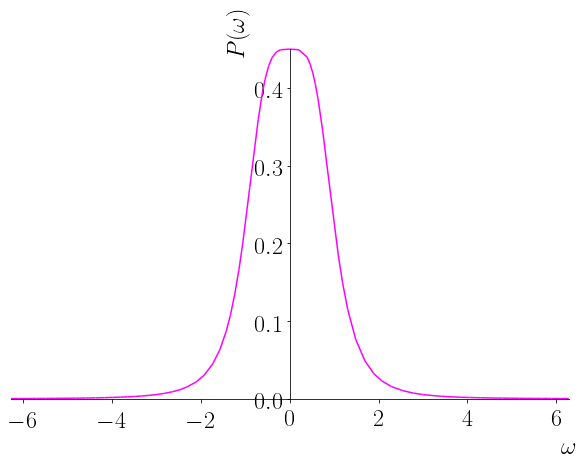
\includegraphics[width=\linewidth]{img/2ldetect/P_omega.png}
    \subcaption{}\label{fig:absorbed-qubit-normalization-loss:omega}
  \end{subfigure}
  \caption[
    Non-unitary evolution of absorbed qubit (cont.)
  ]{
    Non-unitary evolution of absorbed qubit.
    \subref{fig:absorbed-qubit-normalization-loss:t}
      Detection probability in time. It's equal to the
      loss of normalization $-\dv{\norm{\psi}^2}{t}$
      (but also to the squared norm of $\hat{\psi}(t)$ as of Eq.~\eqref{eq:analytic:hatpsi}.
    \subref{fig:absorbed-qubit-normalization-loss:omega}
      Detection probability in the frequency domain.
  }
  \label{fig:absorbed-qubit-normalization-loss}
\end{figure}

The ``lossy'' evolution, with the two components of the qubit, is shown in Fig.~\ref{fig:absorbed-qubit-components}.
The loss of normalization $-\dv{\norm{\psi}^2}{t}$, indicating the probability of arrival in state $\ket{1}$ by absorption,
is then derived directly and shown in Fig.~\ref{fig:absorbed-qubit-normalization-loss}.

This yields the \emph{probability} of detection.
One may wonder whether it is possible to derive a corresponding \emph{probability amplitude} vector,
whose squared norm across time is equal to the said probability distribution.\footnote{
  The solution is of course not unique, but one may ask whether such functions would lead
  to quantum interference patterns and other phenomenology which may be subject of further study.
}
Within the framework of \cite{RuschhauptAbsorption}, a ``wavefunction in time'' in such sense
is the $\hat{\psi}$, as in \eqref{eq:phi_psi_kiukas}.
It is computed in detail within the
notebook in Appendix \ref{detector-model-kiukas-ruschhaupt-schmidt-werner}, Eq.~\eqref{eq:sympy:hatpsi},
simplifying which we obtain:
\begin{equation}\label{eq:analytic:hatpsi}
  \hat{\psi}(t) =
    i 2^{\frac{5}{4}} e^{-\frac{\sqrt{2}}{2}t}\sin(\frac{\sqrt{2}}{2}t) \theta(t)
    \ket{1}
    \text{,}
\end{equation}
with $\theta(t)$ the Heaviside step function.

% \begin{remark}\label{remark:detection_area}
% In general, the operator $\hat{D}$ as in \eqref{eq:schrod_complex_pot}
% is such that the eigen-space corresponding to its zero eigenvalue
% is the ``area'' where the detector is not sensitive. Or, in other words,
% the linear span of states with zero probability of triggering the detector.
% Therefore, when $\hat{D}$ (or its square root) is applied to a state vector,
% for example in \eqref{eq:phi_psi_kiukas},
% the components in such eigenspace are cut off and the resulting
% $\hat{\psi}$, Eq.~\eqref{eq:analytic:hatpsi} in the example, lies at all times in the ``area of detection''
% i.e. it's a multiple of $\ket{1}$ in this case.
% \end{remark}

% Taking the squared modulus, a probability distribution over angular frequency
% (or, equivalently, energy) is obtained:
% \[
%   P(\omega) = \frac{\sqrt{2}}{\pi \left(\omega^{4} + 1\right)}
%   \,\text{.}
% \]
% See Fig. \ref{fig:absorbed-qubit-normalization-loss:omega}.